\documentclass[10pt,a4paper]{report}
\usepackage[latin1]{inputenc}
\usepackage{amsmath}
\usepackage{amsfonts}
\usepackage{amssymb}
\usepackage{graphicx}
\begin{document}
	\begin{titlepage}
		\begin{center}
			\vspace*{1cm}
			
			\textbf{Web Development Continuous Assessment}
			
			\vspace{0.5cm}
			ECM1417
			
			\vspace{1.5cm}
			
			
			\vfill
		
			
			\vspace{0.8cm}
			
			Computer Science\\
			University of Exeter\\
			26/3/2019
			
		\end{center}
	\end{titlepage}

	\newpage
	
	\section{Database}
	Mysql was my chosen database for this coursework. I chose this because it is very common and as such has lots of support and documentation, it is also very easy to learn and we have been learning it in lectures.
	\subsection{Schema}
	For my schema I have decided on 2 tables, one to store data about the stock and one to store data on the users. I have included a user table to simplify the management of user data. The schema of my database is as follows:
	 	\begin{itemize}
	 		\item \textbf{Stock}
	 		\item Stock\_ID: int: Primary Key
	 		\item Stock\_Name: Varchar(50)
	 		\item Amount: int
	 		\item price: double
	 		\item Last\_Modified: timestamp
	 		\item Modified\_by: int: Primary Key
	 		\\
	 		\item \textbf{Users}
	 		\item User\_ID: int: Primary Key
	 		\item Name: Varchar(50)
	 		\item Username: Varchar(50)
	 		\item HashP: binary(50)
	 	\end{itemize}
 	There is a one to many relationship between the User ID column in Users and the Modified by column in Stock. This exists so the website can automatically input the name of the user who modifies the stock making identification and record keeping easier.\\
	\begin{figure}[h]
		\hspace*{-1.6in}
		\centering
		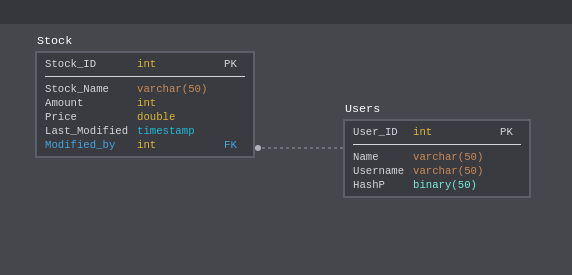
\includegraphics[scale=1]{schema.png}
		\caption{Schema Design}
	\end{figure}
	
	\newpage
	\section{User Interface}
	The user interface is the most vital part of any website, it needs to be clean, easy to look at and intuitive. I have designed my user interface around this idea, I have attempted to make it easy to use and clear enough to be quick to learn.
	\subsection{Font}
	The font I have chosen for my website is roboto slab, a font sourced from fonts.googleapis.com. I chose it for several reason, the main being:
		\begin{itemize}
			\item It is clear and easy to read
			\item It is clean and easy on the eyes
		\end{itemize}
	I have chosen white for the font colour as it contrasts with the background nicely making the text easy to read.
	\begin{figure}
		\centering
		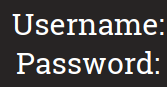
\includegraphics{Font}
		\caption{Font}
	\end{figure}
	
	
	\subsection{Background}
	I have chosen a background colour of hex code \#221F1F as in my experience websites with a darker background and lighter font colour are easier to use and nicer to look at. This sentiment has also began to grow in the tech community with the increase in 'dark theme' implementation and use.
	
	\subsection{Layout}
	\subsubsection{Index.php}
	
	\begin{figure}[h]
		\centering
		\hspace*{-1in}
		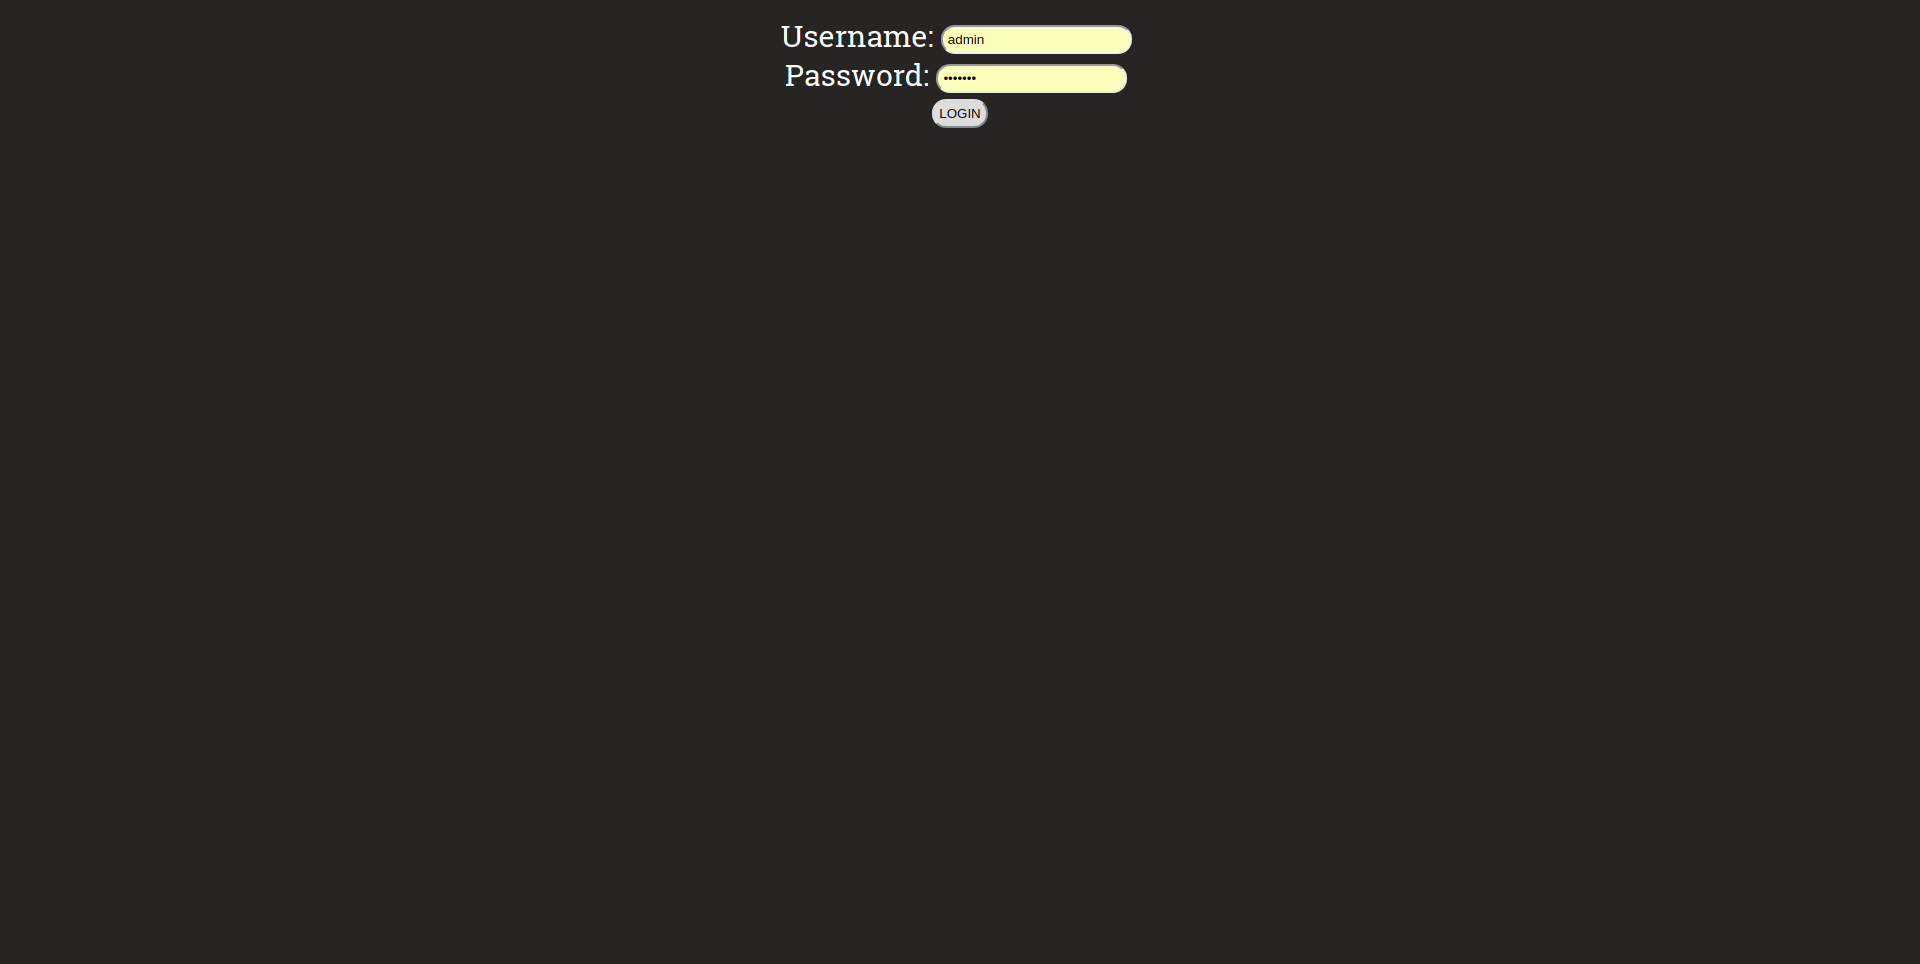
\includegraphics[scale=0.25]{index}
		\caption{Index.php: Login Page}
	\end{figure}

	For the layout of the login page I have kept clutter to a minimum by only having the necessary information displayed. As such only username and passwords tags and input boxes as well as a submit button appear on the page.
	
	I have positioned them at the centre top of the page as it is the most natural position the users eyes will be in upon entering the page.
	
	\newpage
	\subsubsection{Secure.php}
	\begin{figure}[h]
		\centering
		\hspace*{-0.75in}
		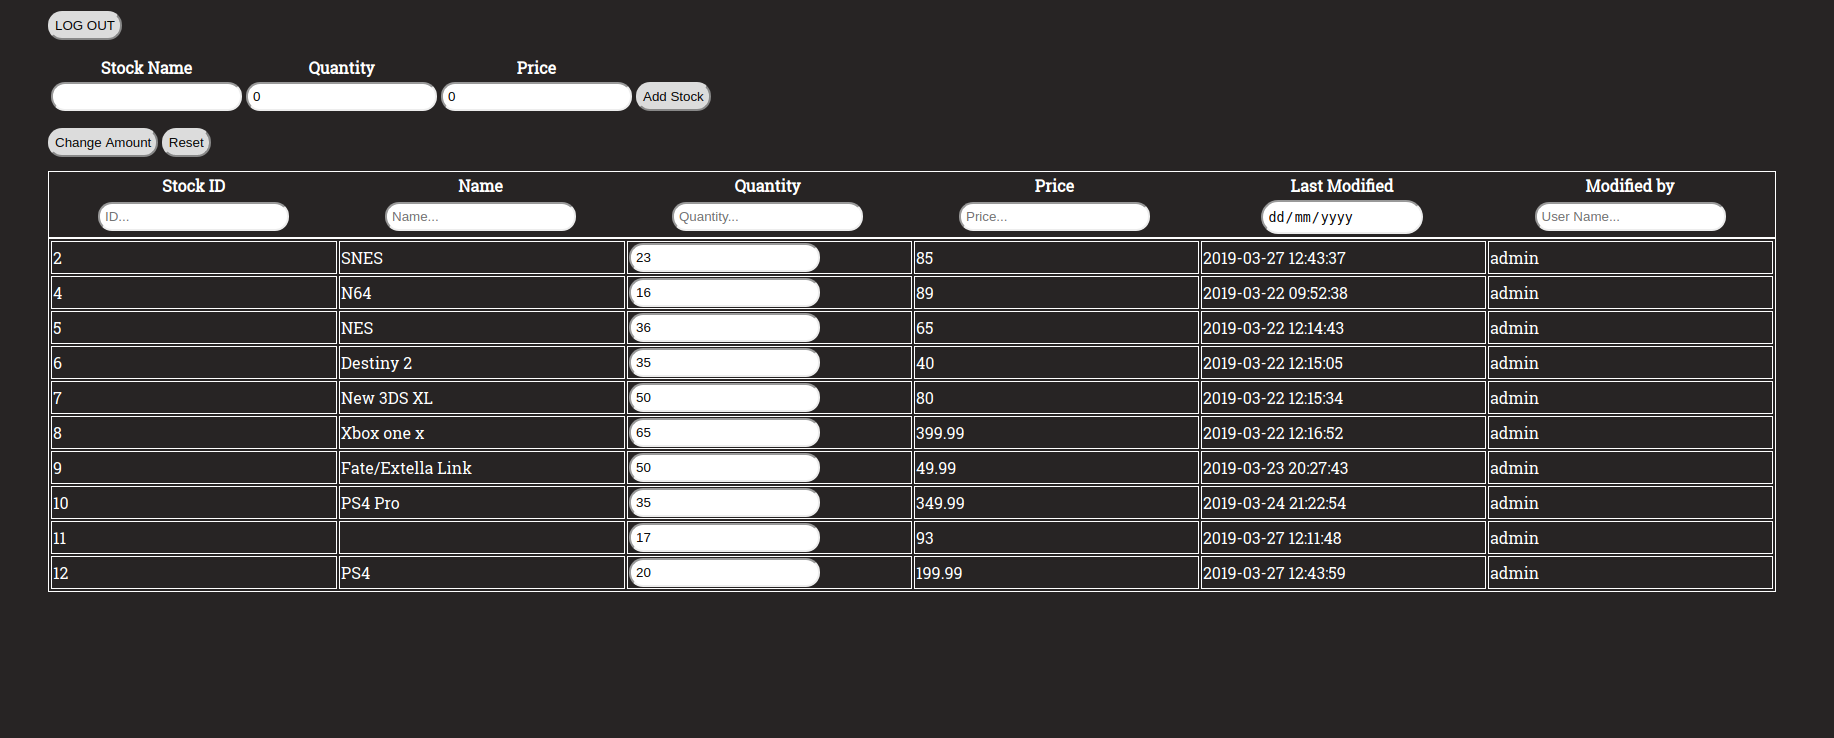
\includegraphics[scale=0.25]{secure}
		\caption{Secure.php: Main Page}
	\end{figure}

	For the main page of this website I have placed the table in the centre of the page with a slight margin on either side. Underneath the titles for each column I have placed search bars which will make quickly assessing stock of specific items easy no matter the size of the table.
	
	Within the Quantity column I have placed number forms for each item of stock. This is to make increasing and decreasing stock easy and intuitive no matter who has to use it. I have placed the submit button above the table however as it makes altering the quantities of multiple stock quick, if I had placed this button at the bottom of the table it would become unreachable once the table grows bigger. I have included a reset button as well which resets the values of all stock to the last submitted value, I have done this so if a mistake is made it can be quickly resolved.
	
	Above the table I have added an area to add stock to the database. Without this adding stock would require sshing into the database and adding it there, something which will be outside the capabilities of most staff.
	
	The logout button has been placed at the top of the page so it is easily identifiable.
	
	\newpage
	\section{Security}
	\subsection{Cross site request forgery}
	In order to counter CSRF I generated a token for the users session which is placed onto any forms the user sends as a hidden input, the php then checks the token to see if it is valid or not. This works as it ensures the user must be logged in order to submit requests.
	
	\subsection{Cross site scripting}
	This can occur whenever you display information to the user. To counter this I used the htmlspecialchars function in php to escape all the character that could cause XSS to occur.
	
	\subsection{Passwords}
	In order to maintain security of passwords I hashed them using bcrypt which stores the hash and the salt together. This can then be placed into the database as one piece of data. This increases the security of the site as it makes it harder to attain the passwords from the database even if the information was leaked.
\end{document}